%% parts/p08/substructural.tex --- Part 8.6
%% Inherited source: v1.1-verified lines 13789--14094.
%% Proof status: the IMLL adequacy/cut item is an inherited sketch and has no
%% compression denominator.  No relevance, exponential-extension, CLL, phase,
%% or Lambek result is promoted into a local proof.
%% OPEN source-exercise obligation: ex:relevance-linear-01 through
%% ex:relevance-linear-04, including their supplied feedback, remain owed in
%% full at exact source-mapped destinations.  The annex sketch, IMLL sheet,
%% apparatus row, and semantic example are separate later material and do not
%% discharge them.

\chapter{Substructural Logics}
\label{sec:p08-substructural}
\chaptermark{Substructural Logics}

\section{Structural policy as logical data}
\label{sec:p08-substructural-policy}

A context is not neutral bookkeeping.  Its representation determines which
changes of order or multiplicity are already identified before any inference
rule is applied.  The comparison below therefore fixes an exact presentation
for every positive cell; it does not classify a whole family from a slogan.

\begin{hbdefinition}{def:p08-context-profile}{Context profile}
For a displayed calculus, its \emph{context profile} is the tuple consisting
of its antecedent or one-sided context representation, whether exchange is
built into that representation, and whether unrestricted weakening and
contraction are available.  This is metalinguistic data about the displayed
calculus, not a new consequence relation.  It is needed because sets erase
order and multiplicity, multisets erase order but retain multiplicity, and
sequences retain both; it differs from a theorem-set inclusion claim.  The
profile is used in Table~\ref{tab:p08-substructural-family} and
Figure~\ref{fig:p08-substructural-family}.
\index{context profile}
\index{structural rule}
\end{hbdefinition}

\section{Relevance logic and ternary semantics}
\label{sec:p08-relevance}

The constant-free relevance language is the least formula set containing the
propositional variables and closed under primitive
\(\neg,\land,\lor,\to\).  Formation alone determines neither a consequence
relation nor a proof calculus.  Two semantic presentations must also be kept
apart: the source's broad pedagogical structures support its calculations,
whereas named systems use source-matched pointed frames.

\begin{hbdefinition}{def:p08-rm-base-structure}{Broad Routley--Meyer structure}
A \emph{broad Routley--Meyer frame} is
\(\mathfrak F=(W,N,R,{*})\), where \(W\ne\varnothing\),
\(\varnothing\ne N\subseteq W\), \(R\subseteq W^3\), star is an involution
on \(W\), and
\[
 n\in N\quad\text{implies}\quad
 \bigl(R(n,u,v)\text{ iff } u=v\bigr).
\]
A corresponding structure is \(\mathcal M=(W,N,R,{*},V)\), with
\(V:\mathsf{Prop}\to\mathcal P(W)\).  Atomic, conjunction, and disjunction
satisfaction have their local clauses, while
\[
 \mathcal M,w\entails\neg A
 \quad\text{ iff }\quad
 \mathcal M,w^*\not\entails A
\]
and
\[
 \begin{aligned}
 \mathcal M,w\entails A\to B
 &\quad\text{ iff }\quad
 \forall u,v\bigl(R(w,u,v)\land\mathcal M,u\entails A\\[-2pt]
 &\hspace{8.5em}\text{ implies }\mathcal M,v\entails B\bigr).
 \end{aligned}
\]
A formula is valid in the structure iff it is satisfied at every member of
\(N\).  The qualifier ``broad'' is necessary: this semantic structure is
strictly less specific than the matched \(\mathbf E\), \(\mathbf R\), and
\(\mathbf{RM}\) frame classes defined below.  Its standing is pedagogical
semantic data, and the distinction is used in all three examples and the
proof boundary.
\index{Routley--Meyer frame}
\index{Routley star}
\end{hbdefinition}

\begin{hbexample}{def:p08-rm-normal-point}{Implication at a broad normal point}
For \(n\in N\), the base condition reduces the implication clause to
\[
 \mathcal M,n\entails A\to B
 \quad\text{ iff }\quad
 \forall u\in W\,
   (\mathcal M,u\entails A\text{ implies }\mathcal M,u\entails B).
\]
Thus the conditional at \(n\) tests global inclusion of truth sets, not merely
the two truth values at \(n\).  At a nonnormal point its ternary coordinate
may test an antecedent at one point and the consequent at another.
\end{hbexample}

\begin{hbexample}{def:p08-rm-star-example}{The star comparison point}
Let \(W=\{w,w^*\}\), let \(N=\{w\}\), let star exchange the two points,
put
\[
 R=\{(w,x,x):x\in W\},\qquad V(p)=\{w\}.
\]
Then \(\mathcal M,w\entails\neg p\), because \(p\) fails at \(w^*\), while
\(\mathcal M,w^*\not\entails\neg p\), because \(p\) holds at \(w\).  This
calculation uses only the displayed broad clauses; it does not assign every
relevance system the same additional negation principles.
\end{hbexample}

\begin{hbexample}{def:p08-rm-irrelevant-weakening}{Failure of irrelevant weakening in the broad structure}
Take four distinct points \(n,a,u,v\), put \(N=\{n\}\), let star be the
identity, and set
\[
 R=\{(n,x,x):x\in\{n,a,u,v\}\}\cup\{(a,u,v)\},
 \qquad V(p)=\{a\},\quad V(q)=\{u\}.
\]
At \(a\), the triple \(R(a,u,v)\) makes \(q\to p\) false.  Since
\(R(n,a,a)\) and \(p\) holds at \(a\),
\[
 \mathcal M,n\not\entails p\to(q\to p).
\]
This refutes irrelevant weakening in the displayed broad structure only; it
does not classify the formula in every system called a relevance logic.
\end{hbexample}

\begin{figure}[!htbp]
\centering
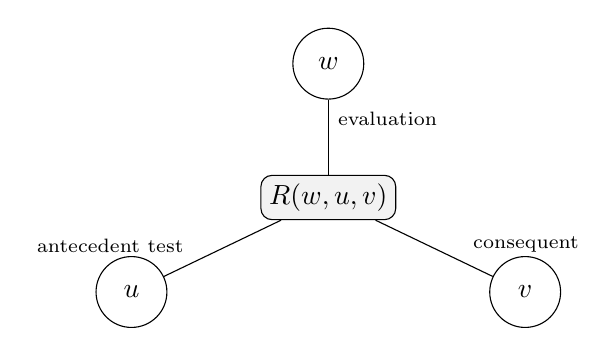
\begin{tikzpicture}[
  world/.style={circle,draw,minimum size=9mm,inner sep=1pt},
  rel/.style={draw,rounded corners,fill=black!5,align=center,
    inner sep=3pt}]
  \node[world] (w) at (0,1.7) {$w$};
  \node[world] (u) at (-2.5,-1.2) {$u$};
  \node[world] (v) at (2.5,-1.2) {$v$};
  \node[rel] (r) at (0,0) {$R(w,u,v)$};
  \draw (w) -- node[right,near start]{\scriptsize evaluation} (r);
  \draw (u) -- node[above left,near start]{\scriptsize antecedent test} (r);
  \draw (v) -- node[above right,near start]{\scriptsize consequent} (r);
\end{tikzpicture}
\caption{One ternary incidence (apparatus A-143).  The three undirected
incidence lines form one hyperedge recording the ordered tuple \(R(w,u,v)\);
they are not binary accessibility arrows.  The implication clause tests
\(A\) at \(u\) and requires \(B\) at \(v\), with \(w\) as its evaluation
coordinate.}
\label{fig:p08-rm-ternary}
\end{figure}

\begin{proofboundary}{def:p08-relevance-proof-boundary}{Broad clauses do not select a relevance calculus}
The broad structure above omits the exact axiom set, inference rules,
derivation objects, hereditary conditions, and matching first-order frame
postulates needed for a soundness or completeness theorem.  The source-scoped
results of Routley and Meyer pair particular calculi with particular ternary
conditions; they are not an adequacy theorem for every structure satisfying
Definition~\ref{def:p08-rm-base-structure} \cite{RoutleyMeyer1972}.
Consequently, no derivability--validity biconditional is inferred from the
broad clauses.  The card below instead uses the separately fixed
\hyperref[sheet:relevance-r]{exact \(\mathbf R\) sheet} and matched pointed
frames.
\index{internal proof boundary!relevance logic}
\end{proofboundary}

\begin{hbdefinition}{def:p08-pointed-rm-frame}{Matched relevance frames}
A \emph{pointed Routley--Meyer frame} is
\(\mathfrak F=(K,R,0,{*})\), with nonempty \(K\), distinguished
\(0\in K\), ternary \(R\), and star on \(K\).  Define
\(a\leq b\) iff \(R(0,a,b)\), and set
\[
\begin{aligned}
 R^2(ab)cd &\quad\text{ iff }\quad
   \exists x\,(R(a,b,x)\land R(x,c,d)),\\
 R^2a(bc)d &\quad\text{ iff }\quad
   \exists x\,(R(b,c,x)\land R(a,x,d)),\\
 R^2b(ac)d &\quad\text{ iff }\quad
   \exists x\,(R(a,c,x)\land R(b,x,d)),\\
 R^2abbc &\quad\text{ iff }\quad
   \exists x\,(R(a,b,x)\land R(x,b,c)).
\end{aligned}
\]
These are metalinguistic abbreviations for composite ternary conditions, not
new accessibility relations.

The cited modular presentation uses the base conditions
\begin{align*}
 \mathrm{B1}:&\ a\leq a,\\
 \mathrm{B2}:&\ a\leq b\land b\leq c\text{ implies }a\leq c,\\
 \mathrm{B3}:&\ a'\leq a\land R(a,b,c)\text{ implies }R(a',b,c),\\
 \mathrm{B4}:&\ a^{**}=a,\\
 \mathrm{B5}:&\ a\leq b\text{ implies }b^*\leq a^*.
\end{align*}
The labels are metalinguistic names for the five displayed frame conditions,
not object-language schemas.  Its \(\mathbf E\)-frames satisfy
B1--B5 and, universally,
\[
\begin{gathered}
 \mathrm{E3}:\ R^2(ab)cd\text{ implies }R^2a(bc)d,\qquad
 \mathrm{E4}:\ R^2(ab)cd\text{ implies }R^2b(ac)d,\\
 \mathrm{E5}:\ R(a,b,c)\text{ implies }R^2abbc,\qquad
 \mathrm{E6}:\ R(a,0,a).
\end{gathered}
\]
Its \(\mathbf R\)-frames are those \(\mathbf E\)-frames also
satisfying \(\mathrm{R7}: R(a,b,c)\text{ implies }R(b,a,c)\).  Its
\(\mathbf{RM}\)-frames additionally satisfy
\(\mathrm{M}: 0\leq a\) or \(0\leq a^*\), for every \(a\).  A valuation is
hereditary along \(\leq\), and the satisfaction clauses are those of
Definition~\ref{def:p08-rm-base-structure}; formula validity is truth at the
distinguished point \(0\).  These are semantic frame classes matched to the
three exact sheets, not the broad class above
\cite{RoutleyMeyer1973,DunnRestall2002}.  A different direct R-frame package
uses period two together with an inversion condition; it is not silently
combined with this modular B1--B5/E3--E6/R7/M presentation.
\index{pointed Routley--Meyer frame}
\end{hbdefinition}

\begin{systementry}{entry:p08-relevance-r}{Relevant implication \(\mathbf R\)}
  \index{relevance logic!R}
  \entryaliases{\(\mathbf R\), the Anderson--Belnap system of relevant
    implication.}
  \entrylanguage{Constant-free formulas over propositional variables, with
    primitive \(\neg,\land,\lor,\to\).}
  \entrysemantics{The matched pointed \(\mathbf R\)-frames of
    Definition~\ref{def:p08-pointed-rm-frame}, with hereditary valuations and
    validity at \(0\).}
  \entrycalculus{sheet:relevance-r}
  \entryadequacy{cited=DunnRestall2002}{Formula theoremhood is sound and
    complete for the matched pointed \(\mathbf R\)-models.  This is not an
    arbitrary-premise local-consequence theorem for the broad frames.}
  \entrydecidability{cited=Urquhart1984}{Full propositional \(\mathbf R\)
    theoremhood is undecidable.  This status does not classify the distinct
    pure implicational fragment; its positive result is stated separately
    below.}
  \entrycharacteristic{It has variable sharing for theorem implications,
    admits Ackermann's theoremhood metarule \(\gamma\), and rejects the
    irrelevant weakening example; these claims retain their separate
    hypotheses below.}
  \entrytranslations{The correspondence cells in
    Table~\ref{tab:p08-relevance-systems} use the composite-relation
    abbreviations of Definition~\ref{def:p08-pointed-rm-frame}.}
  \entrysources{AndersonBelnap1975,RoutleyMeyer1973,DunnRestall2002,Urquhart1984}
\end{systementry}

\begin{hbtheorem}{thm:p08-relevance-adequacy}{cited=DunnRestall2002}{Relevance theoremhood adequacy}
For \(X\in\{\mathbf E,\mathbf R,\mathbf{RM}\}\), let the calculus and
pointed frame class be exactly those fixed by the corresponding registry sheet
and Definition~\ref{def:p08-pointed-rm-frame}.  Then
\[
 \derives_X A\quad\text{ iff }\quad\entails_X A
\]
for formula theoremhood.  The statement does not identify theoremhood with an
arbitrary-premise relevant consequence relation and does not apply to the
broad frames of Definition~\ref{def:p08-rm-base-structure}.
\end{hbtheorem}

\begin{hbtheorem}{thm:p08-relevance-variable-sharing}{cited=AndersonBelnap1975}{Variable sharing for \(\mathbf E\) and \(\mathbf R\)}
Let \(A\) and \(B\) be constant-free formulas.  If
\(\derives_{\mathbf E} A\to B\) or
\(\derives_{\mathbf R} A\to B\), then \(A\) and \(B\) have a propositional
variable in common.  This is a theoremhood property of implications, not an
arbitrary-premise consequence theorem and not a sufficient definition of
relevance.
\end{hbtheorem}

\begin{hbtheorem}{thm:p08-rm-variable-sharing}{cited=DunnRestall2002}{R-mingle and variable sharing}
Full \(\mathbf{RM}\) does not have the variable-sharing property above;
\(\neg(p\to p)\to(q\to q)\) is a standard counterexample.  The safe weaker
statement is: if \(A\to B\) is an \(\mathbf{RM}\)-theorem, then either
\(A\) and \(B\) share a variable, or both \(\neg A\) and \(B\) are
\(\mathbf{RM}\)-theorems.
\end{hbtheorem}

\begin{hbdefinition}{def:p08-ackermann-gamma}{Ackermann's gamma metarule}
Ackermann's \emph{gamma metarule} is the theoremhood-preservation condition
that theoremhood of \(A\) and of \(\neg A\lor B\) entails theoremhood of
\(B\).  Its standing is an admissible metarule, not a primitive object-language
schema or a rule from open assumptions.  The name is necessary to distinguish
this condition from modus ponens, whose conditional premise is \(A\to B\),
and from unrestricted disjunctive syllogism.  It is used in the next theorem
and Table~\ref{tab:p08-relevance-systems}.
\index{Ackermann gamma}
\end{hbdefinition}

\begin{hbtheorem}{thm:p08-gamma-admissibility}{cited=MeyerDunn1969}{Gamma admissibility for \(\mathbf E\) and \(\mathbf R\)}
For \(X\in\{\mathbf E,\mathbf R\}\), if
\(\derives_X A\) and \(\derives_X\neg A\lor B\), then
\(\derives_X B\).  Gamma is not added to either registry sheet: the theorem
says that the metarule preserves theoremhood.  No theory-uniform
\(\mathbf{RM}\) generalization is asserted here.
\end{hbtheorem}

\begin{hbtheorem}{thm:p08-relevance-undecidable}{cited=Urquhart1984}{Undecidability of \(\mathbf E\) and \(\mathbf R\)}
The theoremhood problems for full propositional \(\mathbf E\) and
\(\mathbf R\) are undecidable.  This theorem concerns the full languages; it
does not concern only their pure implicational fragments and supplies no
decision classification for \(\mathbf{RM}\).
\end{hbtheorem}

\begin{hbtheorem}{thm:p08-relevance-implicational-decidable}{cited=DunnRestall2002}{Decidable pure implicational fragments}
The theoremhood problems for the pure implicational fragments
\(\mathbf E_{\to}\) and \(\mathbf R_{\to}\) are decidable.  Their restricted
input languages make this result consistent with
Theorem~\ref{thm:p08-relevance-undecidable}.
\end{hbtheorem}

\begin{hbtheorem}{thm:p08-rm-decidable}{cited=Avron2016}{Decision boundary for \(\mathbf{RM}\)}
Full propositional \(\mathbf{RM}\) is decidable and has the finite-model
property.  This classification is distinct from Urquhart's theorem for
\(\mathbf E\) and \(\mathbf R\) and is also recorded in the standard survey
\cite{DunnRestall2002}.
\end{hbtheorem}

\begin{table}[!htbp]
\centering
\begingroup\scriptsize
\setlength{\tabcolsep}{3pt}
\begin{tabular}{@{}p{.08\textwidth}p{.15\textwidth}p{.15\textwidth}
  p{.23\textwidth}p{.13\textwidth}p{.13\textwidth}@{}}
\toprule
System & Exact sheet & Distinguishing surface & Matched pointed-frame addition
& Variable sharing & Gamma status \\
\midrule
\(\mathbf E\) & \texttt{relevance-e} & Fixed-menu \(\mathbf E\) schemas and
MP/adjunction & Composite associativity/permutation, contraction, point, and
star clauses in Definition~\ref{def:p08-pointed-rm-frame} & yes, for
constant-free theorem implications; Theorem~\ref{thm:p08-relevance-variable-sharing}
& admissible for theoremhood; Theorem~\ref{thm:p08-gamma-admissibility} \\
\(\mathbf R\) & \texttt{relevance-r} & \(\mathbf E\) plus Demodaliser & \(\mathbf E\) conditions plus
  \(R(a,b,c)\text{ implies }R(b,a,c)\) & yes, with the same scope & admissible for
theoremhood \\
\(\mathbf{RM}\) & \texttt{relevance-rm} & \(\mathbf R\) plus Mingle & \(\mathbf R\) conditions plus
\(0\leq a\) or \(0\leq a^*\) & no; weak replacement in
Theorem~\ref{thm:p08-rm-variable-sharing} & no theory-uniform claim; the
package does not promote gamma to a primitive rule \\
\bottomrule
\end{tabular}
\endgroup
\caption{Named relevance systems (apparatus A-087), controlled by
\cite{AndersonBelnap1975,MeyerDunn1969,RoutleyMeyer1973,DunnRestall2002}.
Formula schemas remain exclusively on the named sheets.  ``Gamma'' means the
theoremhood metarule in Definition~\ref{def:p08-ackermann-gamma}, not ordinary
modus ponens.}
\label{tab:p08-relevance-systems}
\end{table}

\section{Inherited IMLL core}
\label{sec:p08-imll}

The inherited calculus has formulas generated from atoms by the tensor unit
\(\mathbf 1\), tensor \(\otimes\), and linear implication
\(\multimap\).  Its sequents have finite-multiset antecedents and exactly one
succedent.  Identity, cut, and every logical rule occur on
\hyperref[sheet:imll]{the IMLL sheet}; exchange is built into multisets, while
weakening and contraction are absent.

\begin{hbdefinition}{def:p08-residuated-pomonoid}{IMLL algebra}
A \emph{commutative residuated partially ordered monoid}, in the inherited
source notation, is
\[
 \mathcal A=(A,\leq,\otimes,1,\multimap),
\]
where \((A,\leq)\) is a partially ordered set,
\((A,\otimes,1)\) is a commutative monoid, tensor is monotone in each
coordinate, and for all \(a,b,c\in A\),
\[
 a\otimes b\leq c\quad\text{ iff }\quad
 b\leq a\multimap c.
\]
This algebraic name is necessary because the IMLL semantics requires one
commutative product, its unit, and its residual but not the lattice operations
used by fuller substructural algebras.  Its standing is an algebraic model
class, not a proof calculus.  Here the locally declared carrier role of \(A\)
is the source's own and overrides its default formula-metavariable role inside
this definition.  The structure is used immediately for sequent validity and
in the IMLL card.
\index{residuated pomonoid}
\end{hbdefinition}

A valuation extends in the source notation by
\[
 \sem{A\otimes B}=\sem A\otimes\sem B,
 \qquad
 \sem{A\multimap B}=\sem A\multimap\sem B,
 \qquad
 \sem{\mathbf1}=1.
\]
The sequent
\(A_1,\ldots,A_n\Rightarrow B\) is valid when
\[
 \sem{A_1}\otimes\cdots\otimes\sem{A_n}\leq\sem B
\]
under every valuation in every such algebra; the empty antecedent tensor is
\(1\).

This paragraph reproduces the controlling inherited v1.1 presentation
verbatim, including its tuple, semantic brackets, and formula-to-algebra
equations.  Galatos et al. are cited below for the broader algebraic class;
their differently typed structure notation is not the controller for this
inherited surface.

\begin{systementry}{entry:p08-imll}{Intuitionistic multiplicative linear logic}
  \index{intuitionistic multiplicative linear logic}
  \entryaliases{\(\mathsf{IMLL}\); the tensor--unit--linear-implication
    core only.}
  \entrylanguage{Atoms, \(\mathbf 1\), \(A\otimes B\), and
    \(A\multimap B\); no additives, exponentials, or primitive linear
    negation.}
  \entrysemantics{Commutative residuated partially ordered monoids, with
    finite-multiset antecedents interpreted by their tensor product.}
  \entrycalculus{sheet:imll}
  \entryadequacy{sketched=annex:p8.imll.1}{The displayed source calculus is sound and
    complete for the displayed algebras, and cut is admissible in its cut-free
    fragment.  The inherited source gives only a proof sketch.}
  \entrydecidability{cited=Lincoln1995}{Derivability for this exact IMLL
    calculus is NP-complete.  NP membership follows from cut elimination and
    the polynomial bound on cut-free IMLL proofs; NP-hardness follows from a
    3-Partition encoding already using only atoms, \(\otimes\), and
    \(\multimap\).}
  \entrycharacteristic{Exchange is built into multiset contexts; unrestricted
    weakening and contraction are absent.}
  \entrytranslations{The source-bounded bang extension below has a distinct
    sheet and does not inherit this card's adequacy status.}
  \entryalgebra{Commutative residuated partially ordered monoids.}
  \entrysources{Girard1987,GalatosJipsenKowalskiOno2007,Lincoln1995}
\end{systementry}

\begin{hbexample}{def:p08-imll-counteralgebra}{Why weakening and contraction fail}
Let \(A=\mathbb Z\), order it by equality, put
\(a\otimes b=a+b\), set \(1^{\mathcal A}=0\), and define
\(a\multimap b=b-a\).  Residuation is the equivalence
\[
 a+b=c\quad\text{ iff }\quad b=c-a.
\]
If \(p\) and \(q\) both receive \(1\), then
\(p\Rightarrow p\otimes p\) would require \(1=2\), so contraction is not
sound.  Likewise \(p,q\Rightarrow p\) would require \(2=1\), so unrestricted
left weakening is not sound.
\end{hbexample}

\begin{proofboundary}{def:p08-imll-bang-boundary}{The source four-rule bang extension}
The source gives the calculus obtained from
\hyperref[sheet:imll]{the IMLL core} by adding formulas \(!A\) and the four
rules on \hyperref[sheet:ill-exponential-extension]{the separate exponential
extension sheet}: dereliction, exponential weakening, exponential contraction,
and promotion with an all-bang antecedent.  Its standing is an unnamed
source-bounded calculus extension, not a new system identifier.  This boundary
is needed to separate those four inherited rules from both multiplicative IMLL
and full intuitionistic linear logic; it adds no
additives or linear negation and is not called full ILL.  No adequacy,
completeness, cut-elimination, or decision result for this extension is
inherited from the source.  This boundary prevents the IMLL sketch from being
transferred to a larger language and is used in
Table~\ref{tab:p08-substructural-family}.
\index{exponential!linear logic}
\end{proofboundary}

\section{Full one-sided classical linear logic}
\label{sec:p08-cll}

The full classical system is independent new depth material.  It does not use
the IMLL annex item as evidence.

\begin{hbdefinition}{def:p08-cll-language}{CLL formulas and linear negation}
The cited one-sided CLL presentation has paired atoms
\(p,p^\perp\), multiplicative units \(\mathbf 1,\bot\), additive units
\(\top,0\), and are closed under
\(\otimes,\bindnasrepma,\mathbin{\&},\oplus,!,?\).  Formula-level
\emph{linear negation} is the involution fixed on atoms and by
\[
\begin{gathered}
 (A\otimes B)^\perp=A^\perp\bindnasrepma B^\perp,
 \qquad
 (A\bindnasrepma B)^\perp=A^\perp\otimes B^\perp,\\
 \mathbf 1^\perp=\bot,\quad \bot^\perp=\mathbf 1,\qquad
 (A\mathbin{\&}B)^\perp=A^\perp\oplus B^\perp,\\
 (A\oplus B)^\perp=A^\perp\mathbin{\&}B^\perp,
 \qquad \top^\perp=0,\quad 0^\perp=\top,\\
 (!A)^\perp=?A^\perp,\qquad(?A)^\perp=!A^\perp.
\end{gathered}
\]
This name is necessary to distinguish an operation on formulas from Routley
star and from phase orthogonality on sets.  Its standing is a syntactic De
Morgan operation, not ordinary object-language falsum; it differs from
primitive negation in the relevance language and is used by the one-sided
sheet, connective table, and phase interpretation.  Linear implication is the
defined connective \(A\multimap B\defeq A^\perp\bindnasrepma B\).
\index{linear negation}
\index{classical linear logic}
\end{hbdefinition}

\begin{hbdefinition}{def:p08-focusing-polarity}{Andreoli focusing polarity}
In Andreoli's one-sided focusing convention used for the displayed CLL
presentation, a formula constructor is
\emph{positive} when its introduction is assigned to a synchronous focused
phase, and \emph{negative} when its introduction is assigned to an
asynchronous phase whose available introduction is invertible.  The positive
nullary connective \(0\) has no introduction rule, so the first clause does
not assert that every positive constructor supplies an applicable rule.  Each
atom receives a declared polarity, and its formal linear negation receives the
opposite polarity.  This is a metalinguistic classification used to schedule
focused proof search, not an object-language connective or a semantic truth
value.  The name is necessary to distinguish the synchronous/asynchronous
proof-search discipline from De Morgan duality and from positive or negative
truth; those classifications do not determine one another.  Table
\ref{tab:p08-linear-connectives} uses the distinction to record the source
constructor classes \cite{Andreoli1992}.
\index{focusing polarity}
\end{hbdefinition}

\begin{table}[!htbp]
\centering
\begingroup\small
\setlength{\tabcolsep}{3pt}
\begin{tabular}{@{}p{.18\textwidth}p{.22\textwidth}p{.19\textwidth}
  p{.14\textwidth}p{.16\textwidth}@{}}
\toprule
Symbol & CLL role & De Morgan dual & Focusing polarity & In IMLL card? \\
\midrule
\(\otimes\) & multiplicative conjunction & \(\bindnasrepma\) & positive & yes \\
\(\bindnasrepma\) & multiplicative disjunction (par) & \(\otimes\) & negative & no \\
\(\mathbf 1\) & tensor unit & \(\bot\) & positive & yes \\
\(\bot\) & par unit & \(\mathbf 1\) & negative & no \\
\(\mathbin{\&}\) & additive conjunction (with) & \(\oplus\) & negative & no \\
\(\oplus\) & additive disjunction (plus) & \(\mathbin{\&}\) & positive & no \\
\(\top\) & with unit & \(0\) & negative & no \\
\(0\) & plus unit & \(\top\) & positive & no \\
\(!\) & bang exponential & \(?\) & positive & no \\
\(?\) & quest exponential & \(!\) & negative & no \\
\(A^\perp\) & formula linear negation & \((A^\perp)^\perp=A\) & reverses
the declared polarity & no primitive counterpart \\
\bottomrule
\end{tabular}
\endgroup
\caption{Linear-logic connective registry (apparatus A-088).  The polarity
column follows Andreoli's focusing convention \cite{Andreoli1992}; it is not
a truth-value classification.  Each atom receives a declared polarity and its
formal negation receives the opposite polarity.}
\label{tab:p08-linear-connectives}
\end{table}

\begin{hbdefinition}{def:p08-phase-space}{Full-CLL phase semantics}
A \emph{phase space}, in Girard's notation, is a pair \((M,\perp)\), where
\(M\) is a commutative monoid written multiplicatively, with unit \(1\), and
\(\perp\subseteq M\) is the \emph{pole}.  For \(X,Y\subseteq M\), define the
phase-subset residual and phase orthogonal by
\[
 X\multimap Y
 =\{m\in M:\forall x\in X\
      (mx\in Y)\},
 \qquad
 X^{\perp}
 =X\multimap\perp.
\]
A \emph{fact} is a subset \(X\subseteq M\) with
\(X=X^{\perp\perp}\).  Here the source uses the same glyph
\({}^{\perp}\) for formula negation and subset orthogonality; the operand type
makes the two roles exact.  These names are needed
to distinguish the semantic model, its designated orthogonality test, and its
closed semantic values from formula-level linear negation.  Here \(\perp\) is
locally typed as a subset of \(M\), not as the formula-level par unit.  Their standing is
semantic: the residual is a typed operation on phase subsets, the pole is a
subset of phases, and a fact is a closed subset, not a formula or a proof
object.  The phase residual differs from formula-level \(\multimap\) by its
subset operands, and is used to define phase orthogonality.  The distinctions
are used in every interpretation clause and in
Theorem~\ref{thm:p08-phase-adequacy}.

Interpret atoms as facts.  Following Girard, write \(A^*\) for the fact
interpreting formula \(A\), and use the connective glyphs themselves for the
corresponding operations on facts:
\[
\begin{aligned}
 X\otimes Y&=\{xy:
                     x\in X, y\in Y\}^{\perp\perp},
 &X\bindnasrepma Y&=(X^\perp\otimes Y^\perp)^\perp,\\
 (\mathbf 1)^*&=\{1\}^{\perp\perp},
 &\bot^*&=\{1\}^{\perp},\\
 X\mathbin{\&}Y&=X\cap Y,
 &X\oplus Y&=(X\cup Y)^{\perp\perp},\\
 \top^*&=M,
 &0^*&=\varnothing^{\perp\perp}.
\end{aligned}
\]
For the exponentials define the idempotent phase set
\[
 I=\{m\in\{1\}^{\perp\perp}:mm=m\},
\]
and set
\[
 !X=(X\cap I)^{\perp\perp},
 \qquad
 ?X=(X^\perp\cap I)^\perp.
\]
The set \(I\) is required for the cited phase interpretation; omitting
it would define only an exponential-free phase semantics.  A formula \(A\) is
\emph{phase-valid} iff \(1\in A^*\) in every such interpretation.  This
validity differs from membership in one phase
model and is the notion used in the next theorem \cite{Girard1995}.
\index{phase semantics}
\index{fact!linear logic}
\end{hbdefinition}

\begin{systementry}{entry:p08-cll}{One-sided classical linear logic}
  \index{classical linear logic!one-sided calculus}
  \entryaliases{\(\mathsf{CLL}\), with full multiplicatives, additives,
    units, and exponentials.}
  \entrylanguage{The formulas and involutive linear negation of
    Definition~\ref{def:p08-cll-language}; one-sided judgments have finite
    multiset contexts.}
  \entrysemantics{The phase models of
    Definition~\ref{def:p08-phase-space}, including the idempotent-phase
    clauses for bang and quest.}
  \entrycalculus{sheet:cll-one-sided}
  \entryadequacy{cited=Girard1995}{Cut is eliminable and formula theoremhood
    is sound and complete for the displayed phase semantics.}
  \entrydecidability{cited=LincolnMitchellScedrovShankar1992}{Full
    propositional CLL is undecidable.  Its exponential-free
    multiplicative--additive fragment is PSPACE-complete, and its
    multiplicative fragment is NP-complete.}
  \entrycharacteristic{No unrestricted weakening or contraction is present;
    the quest-prefixed structural rules are explicit on the sheet.}
  \entrytranslations{\(A\multimap B\defeq
    A^\perp\bindnasrepma B\); the IMLL card is a different, single-succedent
    intuitionistic calculus.}
  \entryalgebra{Phase spaces and their biorthogonally closed facts.}
  \entrysources{Girard1987,Girard1995,Andreoli1992,LincolnMitchellScedrovShankar1992}
\end{systementry}

\begin{hbtheorem}{thm:p08-cll-cut-elimination}{cited=Girard1995}{CLL cut elimination}
Every sequent derivable on \hyperref[sheet:cll-one-sided]{the registered
one-sided CLL sheet} has a cut-free derivation.  Equivalently, its displayed
cut rule is admissible in the cut-free fragment.  This cited theorem covers
the exact multiplicative, additive, unit, and exponential surface of that
sheet; it is not inherited from the IMLL sketch.
\end{hbtheorem}

\begin{hbtheorem}{thm:p08-phase-adequacy}{cited=Girard1995}{Phase soundness and completeness}
For every formula \(A\) in the displayed full propositional CLL language,
\[
 \derives_{\mathsf{CLL}}A
 \quad\text{ iff }\quad
 1\in A^*
 \text{ in every displayed phase interpretation}.
\]
The theorem is formula theoremhood.  The exponential clauses and idempotent
phase set in Definition~\ref{def:p08-phase-space} are part of its hypotheses;
an MALL-only interpretation may not be advertised as this full result.
\end{hbtheorem}

\begin{hbtheorem}{thm:p08-linear-decision-boundaries}{cited=LincolnMitchellScedrovShankar1992}{Linear-logic decision boundaries}
Full propositional linear logic with exponentials is undecidable.  Its
fragment with multiplicatives and additives but no exponentials is
PSPACE-complete, while the multiplicative fragment is NP-complete.  These are
three distinct input languages and do not transfer a decision result to the
source's unnamed four-rule bang extension.
\end{hbtheorem}

\section{The associative Lambek calculus}
\label{sec:p08-lambek}

\begin{hbdefinition}{def:p08-lambek-semantics}{Lambek L and its algebra}
Lambek's \emph{associative calculus \(\mathsf L\)} has formulas
generated from atoms by product \(A\mathbin{\cdot}B\), left division
\(A\backslash B\), and right division \(B/A\).  Antecedents are finite
nonempty ordered sequences; the calculus has no exchange, weakening,
contraction, empty antecedent, or multiplicative unit.  This exact name is
necessary to distinguish \(\mathsf L\) from \(\mathsf L^*\), which permits
empty antecedents, and from \(\mathsf L_1\), which adds a unit.  Its standing
is the proof system on \hyperref[sheet:lambek-l]{the Lambek sheet}, and the
distinction is used in its card and complexity statement.

A \emph{residuated semigroup} is a partially ordered semigroup
\((U,\mathbin{\cdot},\leq)\) with residuals satisfying
\[
 a\mathbin{\cdot}b\leq c
 \quad\text{ iff }\quad
 b\leq a\backslash c
 \quad\text{ iff }\quad
 a\leq c/b.
\]
Its standing is algebraic semantics, not syntax; unlike the IMLL algebra it
need not be commutative or have a unit.  A sequent
\(A_1,\ldots,A_n\Rightarrow B\) is valid iff
\(v(A_1)\mathbin{\cdot}\cdots\mathbin{\cdot}v(A_n)\leq v(B)\) under every
valuation in every such semigroup \cite{Lambek1958,Buszkowski2010}.
\index{Lambek calculus}
\index{residuated semigroup}
\end{hbdefinition}

\begin{systementry}{entry:p08-lambek-l}{Associative Lambek calculus L}
  \index{Lambek calculus!system entry}
  \entryaliases{\(\mathsf L\); unit-free, nonempty-antecedent associative
    Lambek calculus.}
  \entrylanguage{Atoms, product, left division, and right division.}
  \entrysemantics{Residuated semigroups, interpreting the ordered antecedent
    by its left-to-right semigroup product.}
  \entrycalculus{sheet:lambek-l}
  \entryadequacy{cited=Buszkowski2010}{The calculus is sound and complete for
    the displayed residuated-semigroup semantics, and cut is admissible.}
  \entrydecidability{cited=Pentus2006}{Derivability for \(\mathsf L\) is
    NP-complete.  The same cited paper also treats \(\mathsf L^*\), but that is
    not the card's calculus.}
  \entrycharacteristic{Ordered nonempty antecedents make exchange, weakening,
    contraction, and the empty-context unit unavailable.}
  \entrytranslations{Its two residuals coincide only under an additional
    commutativity assumption, which is absent here.}
  \entryalgebra{Partially ordered residuated semigroups without a required
    unit.}
  \entrysources{Lambek1958,Buszkowski2010,Pentus2006}
\end{systementry}

\begin{hbtheorem}{thm:p08-lambek-adequacy}{cited=Buszkowski2010}{Lambek adequacy and cut elimination}
For the exact unit-free, nonempty-antecedent calculus
\hyperref[sheet:lambek-l]{\(\mathsf L\)}, a sequent is derivable iff it is
valid in every residuated semigroup.  Every derivable sequent also has a
cut-free derivation.  Neither assertion silently changes the calculus to
\(\mathsf L^*\) or \(\mathsf L_1\).
\end{hbtheorem}

\section{Comparison by context profile}

\begin{proofboundary}{def:p08-affine-family-boundary}{Affine-family boundary}
In the cited structural classification, an \emph{affine} system admits
unrestricted weakening but not unrestricted contraction.  This is a family
property, not one syntax or calculus: its formula language, context
representation, exchange policy, rules, and semantics must come from the
particular named system.  The distinction is needed to separate weakening
alone from restoration of both classical structural rules.  Because no one
exact cited affine calculus and matching registry sheet is supplied here, the
table and map record only that family property and assert no affine card,
adequacy theorem, or transfer from CLL \cite{Girard1995}.
\index{affine linear logic}
\end{proofboundary}

\begin{table}[!htbp]
\centering
\begingroup\scriptsize
\setlength{\tabcolsep}{3pt}
\begin{tabular}{@{}p{.15\textwidth}p{.19\textwidth}p{.12\textwidth}
  p{.13\textwidth}p{.13\textwidth}p{.20\textwidth}@{}}
\toprule
Named system or boundary & Context representation & Exchange & Unrestricted
weakening & Unrestricted contraction & Exact sheet or boundary \\
\midrule
\(\mathbf E\) & Hilbert theorem sequences, not contexted sequents & not a
structural-rule cell & not a structural-rule cell & not a structural-rule cell
& \hyperref[sheet:relevance-e]{\texttt{relevance-e}} \\
\(\mathbf R\) & Hilbert theorem sequences, not contexted sequents & not a
structural-rule cell & not a structural-rule cell & not a structural-rule cell
& \hyperref[sheet:relevance-r]{\texttt{relevance-r}} \\
\(\mathbf{RM}\) & Hilbert theorem sequences, not contexted sequents & not a
structural-rule cell & not a structural-rule cell & not a structural-rule cell
& \hyperref[sheet:relevance-rm]{\texttt{relevance-rm}} \\
\(\mathsf{IMLL}\) & finite multiset antecedent; one succedent & built in &
absent & absent & \hyperref[sheet:imll]{\texttt{imll}} \\
Source bang extension & finite multiset antecedent; one succedent & built in &
bang-prefixed formulas only & bang-prefixed formulas only &
\hyperref[sheet:ill-exponential-extension]{\texttt{ill-exponential-extension}};
no inherited metatheorem \\
One-sided \(\mathsf{CLL}\) & finite multiset, one-sided & built in &
absent; quest-prefixed exception & absent; quest-prefixed exception &
\hyperref[sheet:cll-one-sided]{\texttt{cll-one-sided}} \\
Affine-family boundary & not fixed by the family name & system-specific &
present & absent & family property only; no sheet, card, or metatheorem \\
Associative Lambek \(\mathsf L\) & finite nonempty ordered antecedent; one
succedent & absent & absent & absent &
\hyperref[sheet:lambek-l]{\texttt{lambek-l}} \\
\bottomrule
\end{tabular}
\endgroup
\caption{Substructural family map by exact context profile (apparatus A-086).
The three relevance rows point separately to their exact Hilbert systems;
assigning them one generic sequent profile would fabricate a calculus.
Exponential weakening and contraction are not unrestricted structural rules.}
\label{tab:p08-substructural-family}
\end{table}

\begin{figure}[!htbp]
\centering
\begin{tikzpicture}[
  profile/.style={draw,rounded corners,align=center,inner sep=5pt,
    text width=3.7cm},
  note/.style={draw,dashed,rounded corners,align=center,inner sep=5pt,
    text width=3.7cm},
  >=Latex]
  \node[profile] (comm) {finite multisets\\exchange built in\\no
    unrestricted weakening or contraction\\\(\mathsf{IMLL}\),
    \(\mathsf{CLL}\)};
  \node[note,right=3.2cm of comm] (aff) {affine-family boundary\\unrestricted
    weakening present\\unrestricted contraction absent\\no single syntax};
  \node[profile,below=2.0cm of comm] (lambek) {nonempty ordered
    sequences\\remove exchange\\associative Lambek \(\mathsf L\)};
  \node[note,below=2.0cm of aff] (rel) {\(\mathbf E,\mathbf R,\mathbf{RM}\)\\
    exact Hilbert sheets\\system-specific; no structural-deletion arrow};
  \draw[dashed,->] (comm) -- node[above,align=center]{family-level
    contrast:\\add weakening}
    (aff);
  \draw[->] (comm) -- node[left,align=right]{retain order;\\remove exchange}
    (lambek);
\end{tikzpicture}
\caption{Structural-policy map (apparatus A-153).  Arrows record only a
change in context policy; they are not theorem-set inclusions, translations,
or claims that one logic is obtained from another merely by deleting an LK
rule.  Formula languages and proof-theoretic standings remain those of the
named sheets.}
\label{fig:p08-substructural-family}
\end{figure}

\section{Consequence properties and scope boundary}
\label{sec:p08-substructural-consequence}

\begin{hbdefinition}{def:p08-context-consequence-properties}{Context-sensitive consequence properties}
For a relation between contexts and conclusions, \emph{identity} means that a
formula follows from its singleton context; \emph{context extension} means
that inserting additional occurrences wherever the declared representation
permits preserves derivability; and \emph{cut composition} means that a
derivation of \(A\) may replace a displayed occurrence of \(A\) in another
derivation.  These are metalinguistic properties of a contexted relation.  They
are needed because Tarskian monotonicity for set-valued semantic consequence
forgets order and multiplicity, whereas the calculi below do not.  Thus context
extension is not renamed ``monotonicity'' in the table, and the distinction is
used to expose the still-missing nonmonotonic half of apparatus A-103.
\index{monotonicity!context extension}
\index{cut!composition}
\end{hbdefinition}

\begin{table}[!htbp]
\centering
\begingroup\scriptsize
\setlength{\tabcolsep}{3pt}
\begin{tabular}{@{}p{.19\textwidth}p{.20\textwidth}p{.13\textwidth}
  p{.19\textwidth}p{.20\textwidth}@{}}
\toprule
Relation or boundary & Representation & Identity & Context extension & Cut /
transitivity standing \\
\midrule
Set-valued semantic consequence & sets of premises & yes & yes, Tarskian
monotonicity & yes, Tarskian transitivity \\
\(\mathsf{IMLL}\) derivability & finite multisets; one succedent & displayed
on \texttt{imll} & no unrestricted extension & cut displayed; elimination
sketched by \hyperref[entry:p08-imll]{the IMLL card} \\
\(\mathsf{CLL}\) derivability & finite one-sided multisets & displayed on the
\hyperref[sheet:cll-one-sided]{CLL sheet} & no unrestricted extension; quest
exception only &
cut displayed and cited eliminable in
Theorem~\ref{thm:p08-cll-cut-elimination} \\
Affine-family boundary & not fixed by the family name & system-specific &
unrestricted weakening is the family property & no independent calculus or
metatheorem asserted here \\
Lambek \(\mathsf L\) derivability & finite nonempty ordered sequences &
displayed on \texttt{lambek-l} & no arbitrary insertion or permutation & cut
displayed and cited eliminable in Theorem~\ref{thm:p08-lambek-adequacy} \\
\(\mathbf E,\mathbf R,\mathbf{RM}\) theoremhood & no premise context in the
exact Hilbert sheets & not a context cell & not a context cell & gamma is a
theoremhood metarule, not structural cut \\
\bottomrule
\end{tabular}
\endgroup
\caption{The exact P8.6 half of the consequence-properties table (apparatus
A-103).  Set monotonicity and occurrence-sensitive context extension are
deliberately separate.}
\label{tab:p08-consequence-properties}
\end{table}

\hbstub{A-103: the P8.6 structural half is complete in Table
\ref{tab:p08-consequence-properties}, but the registered comparison also
requires the P8.7 nonmonotonic systems; that Phase-5 half remains pending, so
the cross-chapter apparatus row stays open.}

\begin{hbwarning}{def:p08-resource-metaphor}{Resource metaphors are not metatheorems}
Calling a formula a ``resource'' may motivate a structural policy, but its
formal content is the declared context representation and the exact rules on
the named sheet.  The metaphor alone establishes no soundness, completeness,
cut-elimination, or complexity claim.
\end{hbwarning}

\hbstub{\texttt{D-P10-030}: coherence spaces and proof nets remain at the
registered pointer ceiling.  No local correctness criterion,
sequentialization theorem, or net-based cut-elimination development is
supplied.}

\begin{proofboundary}{def:p08-linear-pointer-boundary}{Coherence spaces, proof nets, and excluded developments}
Register row \texttt{D-P10-030} receives its pointer-level treatment here:
Girard's coherence-space semantics and proof nets are entry points in the
original linear-logic development \cite{Girard1987}.  The recorded
\hyperref[def:p07-proof-nets-goi-boundary]{Part-7 proof-net and geometry-of-interaction
boundary} governs the scope: no proof-net correctness criterion,
sequentialization theorem, net-based cut elimination, or
geometry-of-interaction execution model is developed.  This preserves
\texttt{N-x-011} and \texttt{N-x-012}.  The separate Part-8 exclusions for
quantum logic, adaptive logics, and formal argumentation
(\texttt{N-x-006}, \texttt{N-x-007}, \texttt{N-x-009}) create no P8.6
theorem obligation.
\index{coherence space}
\index{proof net}
\index{geometry of interaction}
\end{proofboundary}
